\section{X25519与Ed25519}

\subsection{X25519}

RFC 7748中给出了两条蒙哥马利形式的椭圆曲线Curve25519和Curve448,
其中Curve448是Mike Hamburg在2015年设计的新曲线,旨在提供224比特的安全性\footnote{
Hamburg, Mike. Ed448-Goldilocks, a new elliptic curve. IACR Cryptology ePrint Archive 2015 (2015): 625.
\url{https://eprint.iacr.org/2015/625.pdf}}.
本文仅关注Curve25519及定义在其上的ECDH密钥交换协议X25519.
Curve25519是定义在有限域$\F_p, p = 2^{255}-19$的蒙哥马利形式椭圆曲线$y^2 = x^3 + 486662x^2 + x$,
Curve25519的余因子为8,而X25519实际上定义在Curve25519上的子群,阶为\\
\centerline{\texttt{0x1000000000000000000000000000000014def9dea2f79cd65812631a5cf5d3ed},}
RFC 7748中一开始给出的X25519依赖的点群的基点$G$为\\
\centerline{(\texttt{0x9, 0x20ae19a1b8a086b4e01edd2c7748d14c923d4d7e6d7c61b229e9c5a27eced3d9}).}\\
然而在随后的RFC 7748的勘误\footnote{
RFC 7748 Errata. \url{https://www.rfc-editor.org/errata/rfc7748}}
中将基点$G$的具体值修正为\\
\centerline{(\texttt{0x9, 0x5f51e65e475f794b1fe122d388b72eb36dc2b28192839e4dd6163a5d81312c14}).}\\
这是因为, X25519所依赖的椭圆曲线点群运算只涉及点的横坐标,所以X25519涉及的运算只关心横坐标.
然而由于Curve25519与Edwards25519双向有理等价,而Ed25519所依赖的点群运算同时需要横纵坐标,
并且已经有广泛使用的基点的值.
RFC 7748中给出的基点的值,会映射到Edwards25519时会映射成Edwards2519曲线基点的负值,
因此有了上述修正,以便在双向有理映射的条件下保持Edwards25519和Curve25519的基点保持一致.

\begin{figure}[h]
\centering
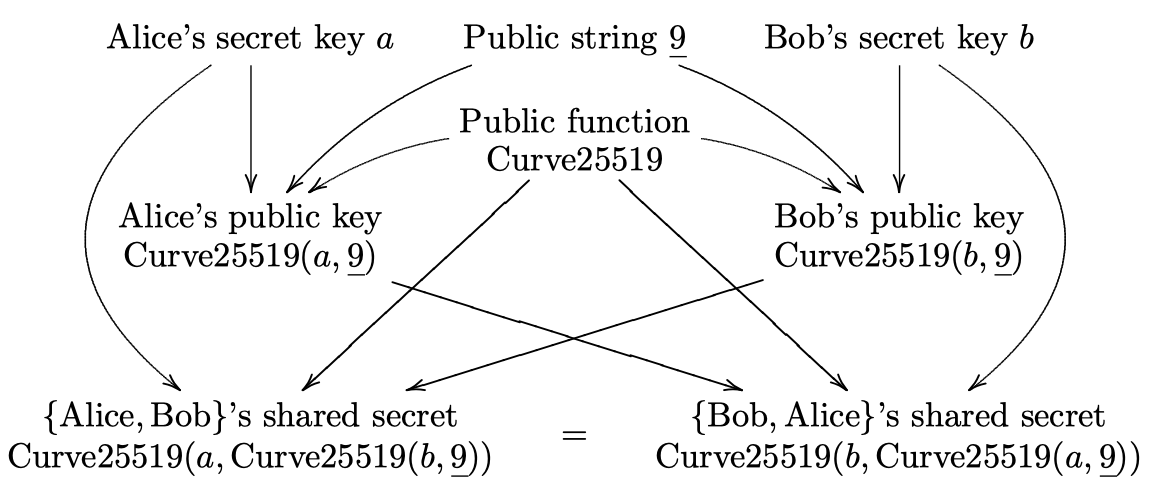
\includegraphics[width=.8\textwidth]{x25519.png}
\caption{X25519密钥交换协议}\label{fig-x25519}
\end{figure}

Alice和Bob之间的ECDH密钥交换协议X25519的执行流程参见Figure~\ref{fig-x25519},
其中'Public string \underline{9}'表示X25519的公共参数基点横坐标的字节数组.
注意这里的点群运算只需要横坐标$x$,用$k$表示标量的话, $x(P)$表示取点$P$的横坐标,
则点的倍乘运算可以表示为$k\cdot x(P)$.
值得提及的是,在X25519和Ed25519的设计文档中,也同时给出了对元素进行编解码的规定.
定义在$\F_p$上的坐标,以小端法编码为字节数组,
也即坐标值$x\in\F_p$与$x[0] + 256  *x[1] + \ldots + 256^{n-1} * x[n-1]$模$p$同余.
从32个字节的数组解码坐标值时,对于X25519协议需要首先将最后一个字节的最高比特位清零,
参见Listing~\ref{lst-x25519-decode}~中第7行,
其中输入参数~\code{bits}~的值为255(对应Curve25519)或者448(对应Curve448).
这个操作的目的是尽可能与基于该曲线的其他协议保持兼容性,因为该比特位通常保留作为标记位.
另外RFC 7748中也明确指出, X25519的协议的实现必须接受非规范(Non-Canonical)的值,
对于X25519而言,非规范的值包括$2^{255}-19$到$2^{255}-1$的所有值.
注意到函数~\code{decodeLittleEndian}~没有对输入参数~\code{u}~做任何限制,
也即32字节的任意值都可以作为Curve25519的公钥$\{\underline{u}, u\in \{0,1,\ldots,2^{256}-1\}\}$.

\begin{lstlisting}[language=python, caption=X25519和X448的编解码, label=lst-x25519-decode]
def decodeLittleEndian(b, bits):
    return sum([ b[i] << 8*i for i in range((bits+7)//8) ])

def decodeUCoordinate(u, bits):
    u_list = [b for b in u]
    # Ignore any unused bits.
    if bits % 8:
        u_list[-1] &= (1 << (bits % 8)) - 1
    return decodeLittleEndian(u_list, bits)

def encodeUCoordinate(u, bits):
    return bytearray([ (u >> 8*i) & 0xff for i in range((bits+7)//8) ])

def decodeScalar25519(k):
    k_list = [b for b in k]
    k_list[0] &= 248  # 1111 1000
    k_list[31] &= 127 # 0111 1111
    k_list[31] |= 64  # 0100 0000
    return decodeLittleEndian(k_list, 255)

def decodeScalar448(k):
    k_list = [b for b in k]
    k_list[0] &= 252
    k_list[55] |= 128
    return decodeLittleEndian(k_list, 448)
\end{lstlisting}

考虑$k\cdot x(P)$中的标量$k$的解析,参见Listing~\ref{lst-x25519-decode}~中的函数~\code{decodeScalar25519}.
与解码坐标值时类似,解码$k$时将32个字节的数组看成是小端法表示的$k$,
但是按照小端法将字节数组转换成标量$k$之前,
需要将最低3比特清零(第16行), 将最高位清零(第17行), 并将紧邻最高位的比特设置为1 (第19行).
也即Curve25519的私钥取值空间为$\{\underline{k}: k\in 2^{254} + 8\cdot\{0,1,\ldots,2^{251}-1\}\}$.
将最低3比特清零可以保证私钥值是8的倍数,考虑到Curve25519曲线的余因子为8,
这样可以避免small-subgroup一类的攻击.
将最高位清零,猜测是为了与公钥的处理方式保持一致.
将紧邻最高位的比特设置为1,有利于常量时间的蒙哥马利阶梯算法实现\footnote{
StackExchange: When using Curve25519, why does the private key always have a fixed bit at 2\^{}254?
\url{https://crypto.stackexchange.com/questions/11810/when-using-curve25519-why-does-the-private-
key-always-have-a-fixed-bit-at-2254/11818\#11818}}.
与secp256k1或者secp256r1等曲线的私钥可以在某个区间内连续取值(整数值)不同,
Curve25519私钥并不是某个区间内的连续取值.
%另外点的倍乘$k\cdot x(P)$可以看做是两个集合到一个集合的映射(非满射):
%$$\{\underline{k}: k\in 2^{254} + 8\cdot\{0,\ldots,2^{251}-1\}\} \times \{\underline{u}, u\in \{0,\ldots,2^{256}-1\}\} \rightarrow \{\underline{u}, u\in \{0,\ldots,2^{256}-1\}\}.$$
%\red{todo: 论证该映射存在的合理性}

前面已经提过到Curve25519上的点群中的加法运算可以仅基于横坐标构建,
第一次见到仅依赖横坐标的点群运算,感觉上非常诡异.
考虑椭圆曲线上点的横坐标与点的关系,可以帮助消除诡异的感觉.
点$P=(x,y)$\textit{基本上}可以仅根据横坐标$x$和曲线方程计算出来,
然而这种计算会得到两个结果$P=(x,y)$以及$-P = (x, -y)$.
由于点和横坐标不是一一对应的,无法通过直接从基于$(x,y)$的点群运算中推导出仅基于横坐标$x$的点群运算.
用$\ominus$表示椭圆曲线$E$上的点的逆映射($\ominus(P) = -P$),定义如下映射$\mathbf{x}$和商群(Quotient Group) $\xi$:
$$\mathbf{x}: E \rightarrow\xi \cong E/\langle\ominus\rangle$$
映射$\mathbf{x}$将$E$中的点送入关于映射$\ominus$的商群$\xi$中:
$$\mathbf{x}(P) = \mathbf{x}(Q) \iff P = Q\ \text{or}\ P = \ominus(Q), P, Q \in E, \mathbf{x}(P), \mathbf{x}(Q) \in \xi.$$
直观上理解, 拥有相同横坐标的点$P, -P$在商群$\xi$中坍缩成同一个元素$\mathbf{x}(P)=\mathbf{x}(-P)$.
并且点$P, -P$的$k$倍乘运算在商群$\xi$中也坍缩成同一个元素.
$$k(-P) = -kP \implies \mathbf{x}(k(-P)) = \mathbf{x}(-kP)= \mathbf{x}(kP).$$
由此, 虽然$\xi$并没有直接从$E$中继承运算,但是签署两个点共享同一个横坐标的问题得到解决,
则$\xi$中可以定义仅依赖于横坐标的运算,并且根据$\xi$和$E$之间的关系,
该运算规则可以根据$E$中的点的加法运算进行推导.
而为了支持高速的ECDH密钥协商,要求能够在$\xi$中根据$\mathbf{x}(P)$和标量$k$快速计算$\mathbf{x}(kP)$.
接下来的问题,就变成了如何构建具有这种形式的椭圆曲线?

蒙哥马利曲线的提出为这一个问题提供了答案,
其中蒙哥马利阶梯(Montgomery Ladder)算法可以根据$\mathbf{x}(P)$和标量$k$快速计算$\mathbf{x}(kP)$,
而蒙哥马利曲线的选择可以保证蒙哥马利阶梯算法中的每一步都可以高效执行.

\begin{figure}[h]
\centering
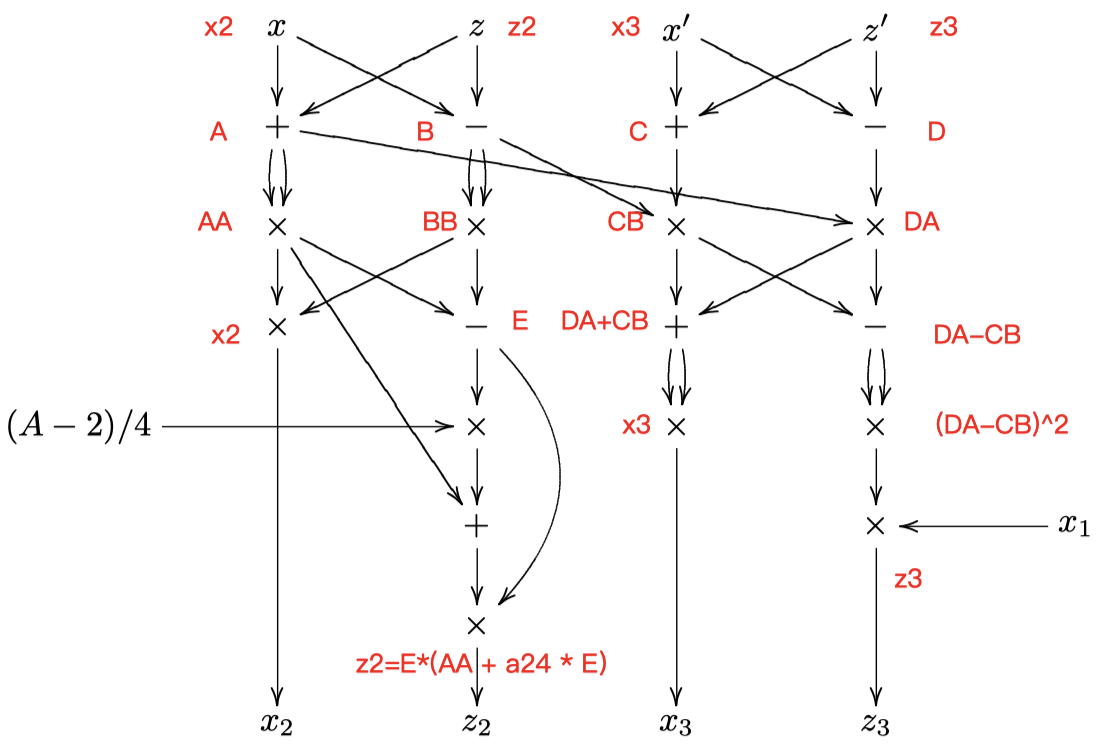
\includegraphics[width=.8\textwidth]{x-coordiniate-add.png}
\caption{X25519密钥交换依赖的点运算}\label{fig-xadd}
\end{figure}

\begin{lstlisting}[language=python, caption = Curve25519和Curve448上的乘法运算, label=lst-curve25519mul]
# Finite field with p
def FiniteField(p):
    class Fp:
        def __init__(self, val: int):
            assert isinstance(val, int)
            self.val = val
        def __add__(self, other):
            return Fp((self.val + other.val) % Fp.p)
        def __sub__(self, other):
            return Fp((self.val - other.val) % Fp.p)
        def __mul__(self, other):
            return Fp((self.val * other.val) % Fp.p)
        def __rmul__(self, n):
            return Fp((self.val * n) % Fp.p)
        def __pow__(self, e):
            return Fp(pow(self.val, e, Fp.p))
        def __repr__(self):
            return hex(self.val)
        def __int__(self):
            return int(self.val)
    Fp.p = p
    return Fp

def cswap(swap, x_2, x_3):
    "Conditional swap in constant time."
    dummy = swap * (x_2 - x_3)
    x_2 = x_2 - dummy
    x_3 = x_3 + dummy
    return x_2, x_3

def mul(k: int, u: int, bits: int, p: int, a24: int):
    Fp = FiniteField(p)
    x_1 = Fp(u)
    x_2 = Fp(1)
    z_2 = Fp(0)
    x_3 = Fp(u)
    z_3 = Fp(1)
    swap = 0

    for t in range(bits-1, -1, -1):
        k_t = (k >> t) & 1
        swap ^= k_t
        (x_2, x_3) = cswap(swap, x_2, x_3)
        (z_2, z_3) = cswap(swap, z_2, z_3)
        swap = k_t

        A = x_2 + z_2
        AA = A**2
        B = x_2 - z_2
        BB = B**2
        E = AA - BB
        C = x_3 + z_3
        D = x_3 - z_3
        DA = D * A
        CB = C * B
        x_3 = (DA + CB)**2
        z_3 = x_1 * (DA - CB)**2
        x_2 = AA * BB
        z_2 = E * (AA + a24 * E)

    x_2, x_3 = cswap(swap, x_2, x_3)
    z_2, z_3 = cswap(swap, z_2, z_3)
    res = x_2 * (z_2**(p - 2))
    return res
\end{lstlisting}

\begin{lstlisting}[language=python, caption = X25519与X448的Python示例, label=lst-x25519x448]
def x25519(k: bytes, u: bytes):
    # Curve25519 for the ~128-bit security level.
    # Computes u := k * u where k is the scalar and u is the u-coordinate.
    bits = 255
    k = decodeScalar25519(k)
    u = decodeUCoordinate(u, bits)
    p = 2**255 - 19
    a24 = 121665
    res = mul(k, u, bits, p, a24)
    return encodeUCoordinate(int(res), bits)

def x448(k: bytes, u: bytes):
    # Curve448 for the ~224-bit security level.
    bits = 448
    k = decodeScalar448(k)
    u = decodeUCoordinate(u, bits)
    p = 2**448 - 2**224 - 1
    a24 = 39081
    res = mul(k, u, bits, p, a24)
    return encodeUCoordinate(int(res), bits)
\end{lstlisting}


Curve25519上的两个不同点的加法运算规则$(x_3, y_3)$

记Curve25519上的两个点$(x_1,y_1), (x_2, y_2)$相加之后得到的点为$(x_3,y_3)$,则